\documentclass[11pt,a4paper]{article}

% ============================================================
% ADGSTUDIOS DISPUTEGUARD
% Production-Grade Card Dispute Management Platform
% ============================================================

\usepackage[margin=2.2cm]{geometry}
\usepackage{amsmath,amssymb,mathtools}
\usepackage{booktabs}
\usepackage{array}
\usepackage{longtable}
\usepackage{enumitem}
\usepackage{xcolor}
\usepackage{hyperref}
\usepackage{graphicx}
\usepackage{float}
\usepackage{listings}
\usepackage{tikz}
\usepackage{pgfplots}
\usepackage{fancyhdr}
\usepackage{titlesec}
\usepackage{microtype}
\usepackage{setspace}
\usepackage{tabularx}

\usetikzlibrary{
    arrows.meta,
    positioning,
    shapes.geometric,
    fit,
    calc
}

\pgfplotsset{compat=1.18}

% ------------------------------------------------------------
% Colours
% ------------------------------------------------------------

\definecolor{ADGBlue}{RGB}{19,67,115}
\definecolor{ADGDark}{RGB}{22,29,38}
\definecolor{ADGLight}{RGB}{239,244,249}
\definecolor{CodeBackground}{RGB}{245,247,249}
\definecolor{CodeGreen}{RGB}{20,110,60}

% ------------------------------------------------------------
% Hyperlinks
% ------------------------------------------------------------

\hypersetup{
    colorlinks=true,
    linkcolor=ADGBlue,
    urlcolor=ADGBlue,
    citecolor=ADGBlue,
    pdftitle={ADGSTUDIOS DisputeGuard Engineering Specification},
    pdfauthor={ADGSTUDIOS}
}

% ------------------------------------------------------------
% Code formatting
% ------------------------------------------------------------

\lstset{
    basicstyle=\ttfamily\small,
    backgroundcolor=\color{CodeBackground},
    frame=single,
    breaklines=true,
    showstringspaces=false,
    keywordstyle=\color{ADGBlue},
    commentstyle=\color{CodeGreen},
    numbers=left,
    numberstyle=\tiny,
    xleftmargin=1.5em,
    framexleftmargin=1em
}

% ------------------------------------------------------------
% Header
% ------------------------------------------------------------

\pagestyle{fancy}
\fancyhf{}
\lhead{\textbf{ADGSTUDIOS}}
\rhead{DisputeGuard}
\cfoot{\thepage}

\setlength{\headheight}{14pt}
\setstretch{1.08}

% ============================================================
% DOCUMENT
% ============================================================

\begin{document}

% ============================================================
% TITLE PAGE
% ============================================================

\begin{titlepage}
    \centering

    \vspace*{2cm}

    {\Huge\bfseries ADGSTUDIOS\par}

    \vspace{0.5cm}

    {\LARGE\color{ADGBlue}\bfseries DisputeGuard\par}

    \vspace{0.5cm}

    {\Large Production-Grade Card Dispute Management Platform\par}

    \vspace{1.5cm}

    \rule{0.85\textwidth}{0.8pt}

    \vspace{1cm}

    {\Large\bfseries Software Engineering Specification\par}

    \vspace{0.5cm}

    {\large
    Full-Stack Banking Technology Demonstration\\
    Rust $\cdot$ Next.js $\cdot$ PostgreSQL $\cdot$ Redis\\
    Ollama $\cdot$ Agentic AI $\cdot$ Docker $\cdot$ Kubernetes
    \par}

    \vfill

    \begin{tabular}{ll}
        \textbf{Organisation:} & ADGSTUDIOS (Pty) Ltd \\
        \textbf{System:} & ADGSTUDIOS DisputeGuard \\
        \textbf{Document Type:} & Engineering / Architecture Specification \\
        \textbf{Version:} & 1.0 \\
        \textbf{Date:} & October 2026 \\
    \end{tabular}

    \vfill

    \textit{
    A secure, auditable and scalable demonstration platform for
    transaction dispute management in a financial-services environment.
    }

\end{titlepage}

\tableofcontents
\newpage

% ============================================================
\section{Executive Summary}
% ============================================================

ADGSTUDIOS DisputeGuard is a production-oriented card dispute
management platform designed to demonstrate the engineering of a
secure financial-services workflow.

The system allows customers to:

\begin{itemize}
    \item authenticate securely;
    \item view mock card transactions;
    \item select eligible transactions;
    \item submit transaction disputes;
    \item provide dispute reasons and supporting evidence;
    \item receive a unique dispute reference;
    \item monitor the dispute lifecycle through a timeline interface.
\end{itemize}

Authorised dispute analysts can:

\begin{itemize}
    \item review incoming disputes;
    \item inspect transaction information;
    \item inspect mathematical risk indicators;
    \item review customer evidence;
    \item request additional information;
    \item transition disputes through controlled states;
    \item use AI-assisted case summarisation;
    \item approve or reject cases according to authorised workflow rules;
    \item inspect a complete audit trail.
\end{itemize}

The core system is intentionally designed so that deterministic business
logic remains independent of generative artificial intelligence.

The design principle is:

\[
\boxed{
\text{Mathematics Computes}
\rightarrow
\text{Software Enforces}
\rightarrow
\text{AI Assists}
\rightarrow
\text{Humans Decide}
}
\]

The proposed technology stack consists of:

\begin{itemize}
    \item Next.js and TypeScript for the user interfaces;
    \item Rust, Axum and Tokio for the backend API;
    \item PostgreSQL as the authoritative transactional datastore;
    \item Redis for caching, rate limiting and asynchronous coordination;
    \item Ollama for locally controlled LLM inference;
    \item an agentic bounded investigation loop for AI assistance;
    \item Docker for reproducible execution;
    \item Kubernetes as an optional production-style deployment model.
\end{itemize}

% ============================================================
\section{Project Objectives}
% ============================================================

The primary objectives are:

\begin{enumerate}
    \item Implement the required card-dispute workflow completely.
    \item Demonstrate production-quality software engineering.
    \item Protect transaction and dispute information through explicit
          authorisation rules.
    \item Prevent duplicate and invalid dispute operations.
    \item Maintain a traceable dispute history.
    \item Demonstrate mathematical risk analysis.
    \item Demonstrate safe AI augmentation without delegating financial
          decisions to an LLM.
    \item Provide automated testing and reproducible deployment.
    \item Demonstrate horizontal scalability without making Kubernetes
          necessary for local execution.
\end{enumerate}

% ============================================================
\section{Scope}
% ============================================================

\subsection{Required Scope}

The minimum functional system shall provide:

\begin{enumerate}
    \item mock transaction retrieval;
    \item transaction presentation;
    \item dispute submission;
    \item persistent dispute storage;
    \item dispute status management;
    \item dispute timeline visualisation.
\end{enumerate}

\subsection{Extended Scope}

DisputeGuard extends the minimum implementation with:

\begin{itemize}
    \item authentication;
    \item role-based access control;
    \item customer ownership validation;
    \item evidence handling;
    \item analyst workflows;
    \item audit logging;
    \item deterministic risk scoring;
    \item statistical anomaly indicators;
    \item AI-assisted classification;
    \item AI-assisted summarisation;
    \item bounded agent execution;
    \item Redis-backed asynchronous jobs;
    \item structured logging;
    \item metrics;
    \item Docker Compose;
    \item Kubernetes manifests;
    \item CI/CD support.
\end{itemize}

% ============================================================
\section{System Actors}
% ============================================================

The primary actors are:

\begin{longtable}{p{0.22\textwidth}p{0.68\textwidth}}
\toprule
\textbf{Actor} & \textbf{Responsibilities} \\
\midrule

Customer &
Views their own transactions, creates disputes, uploads supporting
evidence and monitors case progress. \\

Dispute Analyst &
Reviews assigned or queued disputes, examines risk signals, requests
evidence, records notes and performs authorised transitions. \\

Administrator &
Manages administrative configuration and authorised users. \\

AI Worker &
Performs bounded classification, summarisation and investigation-assist
operations. It cannot make final financial decisions. \\

System &
Enforces authentication, authorisation, state transitions, persistence,
auditability, rate limits and integrity constraints. \\

\bottomrule
\end{longtable}

% ============================================================
\section{High-Level Architecture}
% ============================================================

\begin{figure}[H]
\centering

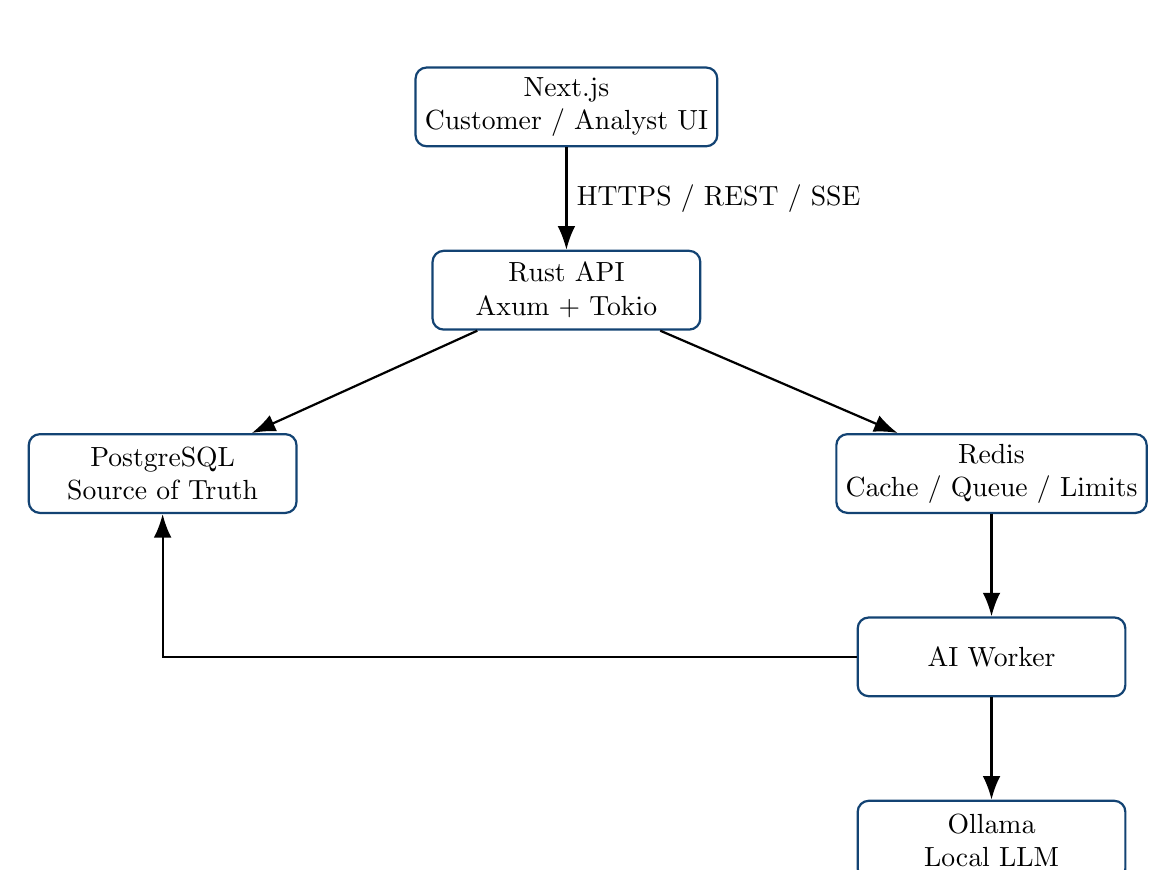
\begin{tikzpicture}[
    node distance=1.3cm and 1.7cm,
    box/.style={
        rectangle,
        rounded corners,
        draw=ADGBlue,
        thick,
        minimum width=3.4cm,
        minimum height=1cm,
        align=center
    },
    arrow/.style={-{Latex[length=3mm]}, thick}
]

\node[box] (web) {Next.js\\Customer / Analyst UI};
\node[box, below=of web] (api) {Rust API\\Axum + Tokio};

\node[box, below left=of api] (postgres) {PostgreSQL\\Source of Truth};
\node[box, below right=of api] (redis) {Redis\\Cache / Queue / Limits};

\node[box, below=of redis] (worker) {AI Worker};
\node[box, below=of worker] (ollama) {Ollama\\Local LLM};

\draw[arrow] (web) -- node[right]{HTTPS / REST / SSE} (api);
\draw[arrow] (api) -- (postgres);
\draw[arrow] (api) -- (redis);
\draw[arrow] (redis) -- (worker);
\draw[arrow] (worker) -- (ollama);
\draw[arrow] (worker.west) -| (postgres.south);

\end{tikzpicture}

\caption{High-level DisputeGuard architecture.}
\end{figure}

% ============================================================
\section{Frontend Architecture}
% ============================================================

The frontend shall be implemented using Next.js and TypeScript.

The application contains two primary workspaces.

\subsection{Customer Workspace}

The customer interface provides:

\begin{itemize}
    \item login;
    \item dashboard;
    \item transaction history;
    \item transaction details;
    \item dispute eligibility;
    \item dispute creation wizard;
    \item evidence submission;
    \item dispute history;
    \item status timeline.
\end{itemize}

\subsection{Analyst Workspace}

The analyst interface provides:

\begin{itemize}
    \item case queue;
    \item filters;
    \item priority ordering;
    \item case details;
    \item transaction details;
    \item risk analysis;
    \item evidence viewer;
    \item analyst notes;
    \item AI case summary;
    \item controlled state transitions;
    \item audit event viewer.
\end{itemize}

% ============================================================
\section{Backend Architecture}
% ============================================================

The backend shall be written in Rust.

Recommended libraries include:

\begin{itemize}
    \item Axum for HTTP routing;
    \item Tokio for asynchronous execution;
    \item SQLx for PostgreSQL access;
    \item Serde for serialisation;
    \item Tower middleware;
    \item Tracing for structured telemetry.
\end{itemize}

The backend should use a layered architecture:

\[
\text{HTTP}
\rightarrow
\text{Application}
\rightarrow
\text{Domain}
\rightarrow
\text{Infrastructure}.
\]

The domain layer shall not depend directly upon HTTP, Redis or
PostgreSQL implementation details.

% ============================================================
\section{Proposed Repository Structure}
% ============================================================

\begin{lstlisting}
ADG-DisputeGuard/
|
|-- apps/
|   |-- web/
|   |-- api/
|   `-- ai-worker/
|
|-- crates/
|   |-- domain/
|   |-- application/
|   |-- persistence/
|   `-- common/
|
|-- database/
|   |-- migrations/
|   `-- seeds/
|
|-- infrastructure/
|   |-- docker/
|   `-- kubernetes/
|
|-- docs/
|   |-- specification.tex
|   |-- threat-model.md
|   `-- diagrams/
|
|-- tests/
|
|-- docker-compose.yml
|-- Dockerfile
|-- README.md
`-- .github/workflows/
\end{lstlisting}

% ============================================================
\section{Domain Model}
% ============================================================

Let:

\[
\mathcal{U} = \text{set of users},
\]

\[
\mathcal{C} = \text{set of cards},
\]

\[
\mathcal{T} = \text{set of transactions},
\]

and

\[
\mathcal{D} = \text{set of disputes}.
\]

A transaction is represented by:

\[
t =
(
id,
customer,
card,
merchant,
amount,
currency,
timestamp,
status
).
\]

A dispute is represented by:

\[
d =
(
id,
transaction,
customer,
reason,
status,
createdAt,
updatedAt
).
\]

% ============================================================
\section{Database Design}
% ============================================================

Core tables include:

\begin{itemize}
    \item users;
    \item cards;
    \item transactions;
    \item disputes;
    \item dispute\_events;
    \item dispute\_evidence;
    \item analyst\_notes;
    \item audit\_logs;
    \item ai\_analysis;
\end{itemize}

\subsection{Important Relationships}

\[
User \rightarrow Card
\]

\[
Card \rightarrow Transaction
\]

\[
Transaction \rightarrow Dispute
\]

\[
Dispute \rightarrow DisputeEvent
\]

\[
Dispute \rightarrow Evidence
\]

\[
Dispute \rightarrow AIAnalysis.
\]

% ============================================================
\section{Financial Data Representation}
% ============================================================

Floating-point arithmetic shall not be used for authoritative monetary
values.

For currency with two decimal places, an amount may be represented in
minor units:

\[
R1234.56 \rightarrow 123456.
\]

Therefore:

\[
amount_{\text{minor}} \in \mathbb{Z}.
\]

Alternatively, a fixed precision PostgreSQL numeric type may be used.

This avoids binary floating-point representation errors such as:

\[
0.1 + 0.2 \neq 0.3
\]

under standard binary floating-point arithmetic.

% ============================================================
\section{Dispute State Machine}
% ============================================================

Let the state space be:

\[
S =
\{
SUBMITTED,
UNDER\_REVIEW,
EVIDENCE\_REQUIRED,
EVIDENCE\_RECEIVED,
INVESTIGATING,
APPROVED,
REJECTED,
REFUND\_PENDING,
RESOLVED
\}.
\]

Let:

\[
E = \text{set of authorised dispute events}.
\]

Define the transition function:

\[
T:S\times E\rightarrow S\cup\{\bot\}.
\]

Here,

\[
\bot
\]

denotes an invalid transition.

Examples include:

\[
T(SUBMITTED,BEGIN\_REVIEW)
=
UNDER\_REVIEW,
\]

\[
T(UNDER\_REVIEW,REQUEST\_EVIDENCE)
=
EVIDENCE\_REQUIRED,
\]

\[
T(EVIDENCE\_REQUIRED,EVIDENCE\_SUBMITTED)
=
EVIDENCE\_RECEIVED,
\]

\[
T(INVESTIGATING,APPROVE)
=
APPROVED,
\]

and

\[
T(INVESTIGATING,REJECT)
=
REJECTED.
\]

An invalid transition is represented by:

\[
T(SUBMITTED,ISSUE\_REFUND)
=
\bot.
\]

The backend shall reject any transition for which:

\[
T(s,e)=\bot.
\]

% ============================================================
\section{Duplicate Dispute Prevention}
% ============================================================

Define the set of active dispute states as:

\[
S_A \subseteq S.
\]

The system invariant is:

\[
\forall t\in\mathcal{T},
\quad
\left|
\{
d\in\mathcal{D}
:
d.transaction=t
\land
d.status\in S_A
\}
\right|
\leq 1.
\]

This invariant shall be enforced primarily by PostgreSQL rather than by
Redis.

The API may perform an early existence check for user experience, but
database-level enforcement remains authoritative.

% ============================================================
\section{Authentication and Authorisation}
% ============================================================

Define:

\[
Owner(u,t)
\]

to mean user \(u\) owns the account/card associated with transaction
\(t\).

Then:

\[
CanViewTransaction(u,t)
\iff
Owner(u,t)
\lor
Role(u)\in\{ANALYST,ADMIN\}.
\]

For customer dispute creation:

\[
CanDispute(u,t)
\Rightarrow
Owner(u,t).
\]

An identifier supplied by the browser shall never establish ownership.

The backend shall independently verify:

\[
transaction.customer\_id
=
authenticated\_user.id.
\]

% ============================================================
\section{Role-Based Access Control}
% ============================================================

Define roles:

\[
R =
\{
CUSTOMER,
ANALYST,
ADMIN
\}.
\]

Permissions shall be explicit.

For example:

\[
P(CUSTOMER)
=
\{
VIEW\_OWN\_TRANSACTION,
CREATE\_OWN\_DISPUTE,
VIEW\_OWN\_DISPUTE
\}.
\]

\[
P(ANALYST)
=
P(CUSTOMER)
\cup
\{
VIEW\_CASE,
REVIEW\_CASE,
REQUEST\_EVIDENCE,
TRANSITION\_CASE
\}.
\]

Administrative privileges shall not implicitly be exposed through
frontend controls alone; they shall be verified server-side.

% ============================================================
\section{Idempotency}
% ============================================================

Financial APIs must tolerate retries.

For dispute creation, the client may supply:

\[
K = \text{Idempotency-Key}.
\]

The server stores:

\[
(K,u,h,r),
\]

where:

\begin{itemize}
    \item \(K\) is the key;
    \item \(u\) is the authenticated user;
    \item \(h\) is a hash of the request;
    \item \(r\) is the original result.
\end{itemize}

If the same request is retried:

\[
(K,u,h)=(K',u',h'),
\]

the original result is returned.

If the key is reused with a different payload:

\[
K=K'
\land
h\neq h',
\]

the request shall be rejected.

% ============================================================
\section{Optimistic Concurrency}
% ============================================================

A dispute shall contain a version:

\[
v_d \in \mathbb{N}.
\]

An update is permitted only if:

\[
v_{\text{request}}
=
v_{\text{database}}.
\]

After successful mutation:

\[
v_{new}=v_{old}+1.
\]

Conceptually:

\begin{lstlisting}[language=SQL]
UPDATE disputes
SET status = $1,
    version = version + 1
WHERE id = $2
  AND version = $3;
\end{lstlisting}

If zero rows are updated, a concurrent modification has occurred.

% ============================================================
\section{Audit Model}
% ============================================================

Every security-sensitive or case-sensitive operation shall produce an
audit event.

An audit event may be represented as:

\[
a =
(
actor,
action,
resource,
timestamp,
metadata
).
\]

For state changes, store:

\[
(s_{old},s_{new},actor,timestamp).
\]

The audit history shall be append-oriented.

Application users shall not be permitted to silently rewrite historical
audit events.

% ============================================================
\section{Mathematical Risk Engine}
% ============================================================

The mathematical risk engine provides deterministic signals for analyst
triage.

It does \textbf{not} determine whether fraud occurred.

For dispute \(d\), define:

\[
R(d)
=
w_A A(d)
+
w_V V(d)
+
w_M M(d)
+
w_H H(d)
+
w_G G(d),
\]

where:

\[
w_i\geq0
\]

and

\[
\sum_i w_i=1.
\]

The components represent:

\begin{align*}
A(d) &= \text{amount anomaly},\\
V(d) &= \text{transaction velocity anomaly},\\
M(d) &= \text{merchant risk signal},\\
H(d) &= \text{historical behaviour anomaly},\\
G(d) &= \text{geographical anomaly}.
\end{align*}

Therefore:

\[
0\leq R(d)\leq1
\]

provided every component lies in \([0,1]\).

% ============================================================
\section{Amount Normalisation}
% ============================================================

Raw monetary values may have highly skewed distributions.

A logarithmic transformation may therefore be used:

\[
A(x)
=
\min
\left(
1,
\frac{\ln(1+x)}
{\ln(1+x_{\max})}
\right).
\]

This reduces domination by extremely large values.

% ============================================================
\section{Statistical Transaction Anomaly}
% ============================================================

For customer \(u\), suppose historical transaction amounts are:

\[
x_1,x_2,\ldots,x_n.
\]

The sample mean is:

\[
\bar{x}_u
=
\frac{1}{n}
\sum_{i=1}^{n}x_i.
\]

The sample variance is:

\[
s_u^2
=
\frac{1}{n-1}
\sum_{i=1}^{n}
(x_i-\bar{x}_u)^2.
\]

Therefore:

\[
s_u
=
\sqrt{
\frac{1}{n-1}
\sum_{i=1}^{n}
(x_i-\bar{x}_u)^2
}.
\]

For new transaction \(x\):

\[
z_x
=
\frac{x-\bar{x}_u}{s_u}.
\]

The magnitude:

\[
|z_x|
\]

provides a simple indication of how unusual the transaction amount is
relative to the customer's historical behaviour.

For demonstration purposes:

\[
|z_x|>3
\]

may be labelled highly unusual.

This is an anomaly indicator, not proof of fraud.

% ============================================================
\section{Robust Statistics}
% ============================================================

Transaction distributions are frequently non-normal and contain
outliers.

A robust alternative uses the median:

\[
m = median(x_1,\ldots,x_n)
\]

and Median Absolute Deviation:

\[
MAD
=
median(|x_i-m|).
\]

A modified z-score can be defined as:

\[
z_i^{*}
=
\frac{0.6745(x_i-m)}{MAD}.
\]

This is less sensitive to extreme historical transactions than the
ordinary mean and standard deviation.

% ============================================================
\section{Transaction Velocity}
% ============================================================

Let:

\[
N_u(t-\Delta t,t)
\]

represent the number of transactions made by customer \(u\) during
window \((t-\Delta t,t]\).

Define transaction velocity:

\[
V_u(t)
=
\frac{N_u(t-\Delta t,t)}{\Delta t}.
\]

Suppose historical velocity has mean:

\[
\mu_{V,u}
\]

and standard deviation:

\[
\sigma_{V,u}.
\]

Then:

\[
z_V
=
\frac{V_u(t)-\mu_{V,u}}
{\sigma_{V,u}}.
\]

Large positive values indicate unusually high transaction frequency.

% ============================================================
\section{Geographical Analysis}
% ============================================================

For two geographic points:

\[
(\phi_1,\lambda_1)
\]

and

\[
(\phi_2,\lambda_2),
\]

the Haversine formula gives:

\[
a
=
\sin^2
\left(
\frac{\Delta\phi}{2}
\right)
+
\cos(\phi_1)
\cos(\phi_2)
\sin^2
\left(
\frac{\Delta\lambda}{2}
\right).
\]

Then:

\[
c
=
2
\arctan2
\left(
\sqrt{a},
\sqrt{1-a}
\right).
\]

Distance is:

\[
d=R_Ec,
\]

where approximately:

\[
R_E=6371\text{ km}.
\]

If the elapsed time is:

\[
\Delta t,
\]

the implied travel velocity is:

\[
v_{required}
=
\frac{d}{\Delta t}.
\]

An implausibly large value may contribute to a geographical anomaly
signal.

However, merchant location, online payments, VPN usage, delayed
settlement and travel must prevent this signal from being interpreted
as proof of fraud.

% ============================================================
\section{Risk Interpretation}
% ============================================================

For presentation purposes only, risk scores may be divided into
bands:

\[
0\leq R<0.30
\Rightarrow LOW,
\]

\[
0.30\leq R<0.60
\Rightarrow MODERATE,
\]

\[
0.60\leq R<0.80
\Rightarrow HIGH,
\]

\[
0.80\leq R\leq1
\Rightarrow VERY\ HIGH.
\]

These thresholds shall be configuration values rather than hard-coded
financial policy.

% ============================================================
\section{AI Architecture}
% ============================================================

Ollama shall provide local model inference.

Permitted AI use cases include:

\begin{itemize}
    \item dispute classification;
    \item customer-description summarisation;
    \item analyst case summarisation;
    \item evidence recommendations;
    \item investigation assistance.
\end{itemize}

AI shall not:

\begin{itemize}
    \item approve a dispute;
    \item reject a dispute;
    \item issue a refund;
    \item change balances;
    \item bypass RBAC;
    \item access arbitrary customer information;
    \item execute unrestricted database queries.
\end{itemize}

The central invariant is:

\[
AIRecommendation(d)
\not\Rightarrow
FinalDecision(d).
\]

Instead:

\[
FinalDecision(d)
\Rightarrow
AuthorisedHumanAction(d).
\]

% ============================================================
\section{Structured AI Output}
% ============================================================

AI responses shall use structured schemas wherever possible.

Example:

\begin{lstlisting}
{
  "suggested_category": "DUPLICATE_TRANSACTION",
  "confidence": 0.91,
  "summary": "Customer reports duplicate billing.",
  "priority": "NORMAL",
  "recommended_evidence": [
    "Merchant receipt",
    "Order confirmation"
  ]
}
\end{lstlisting}

The backend shall validate model output before persistence.

Invalid output shall be discarded or marked as failed analysis.

% ============================================================
\section{Bounded Agentic Investigation Loop}
% ============================================================

The optional investigation agent follows a bounded iterative pattern.

Let the agent state at iteration \(k\) be:

\[
A_k
=
(C_k,O_k,B_k),
\]

where:

\[
C_k = \text{current case context},
\]

\[
O_k = \text{observations obtained through authorised tools},
\]

and

\[
B_k = \text{remaining execution budget}.
\]

The next state is:

\[
A_{k+1}
=
F(A_k,\tau_k),
\]

where:

\[
\tau_k
\in
\mathcal{T}_{allowed}
\]

is an approved tool call.

The loop terminates when:

\[
Complete(A_k)=true,
\]

or when any resource constraint is reached.

% ============================================================
\section{Agent Safety Bounds}
% ============================================================

Let:

\[
k_{\max}
\]

be the maximum number of reasoning iterations.

Then:

\[
k\leq k_{\max}.
\]

Similarly:

\[
N_{tools}\leq N_{tools}^{max},
\]

\[
N_{tokens}\leq N_{tokens}^{max},
\]

and

\[
T_{execution}\leq T_{max}.
\]

Therefore termination is guaranteed by bounded execution even if the
model repeatedly requests additional actions.

A possible demonstration configuration is:

\[
k_{\max}=8.
\]

% ============================================================
\section{AI Tool Allowlist}
% ============================================================

Possible read-only tools include:

\begin{itemize}
    \item get\_transaction;
    \item get\_customer\_transaction\_summary;
    \item get\_dispute\_timeline;
    \item get\_evidence\_metadata;
    \item get\_risk\_signals;
    \item get\_merchant\_summary.
\end{itemize}

The agent shall not receive a generic SQL execution tool.

Formally:

\[
\tau_k
\in
\mathcal{T}_{allowed}.
\]

If:

\[
\tau_k
\notin
\mathcal{T}_{allowed},
\]

execution shall be rejected.

% ============================================================
\section{AI Explainability}
% ============================================================

The interface shall not attempt to expose private model chain-of-thought.

Instead, the system records structured execution events such as:

\begin{lstlisting}
{
  "step": 3,
  "action": "get_risk_signals",
  "result": "high_amount_anomaly",
  "next": "request_manual_review"
}
\end{lstlisting}

The analyst receives:

\begin{itemize}
    \item deterministic mathematical signals;
    \item tool execution history;
    \item concise AI-generated summary;
    \item AI confidence metadata where applicable.
\end{itemize}

% ============================================================
\section{Redis Design}
% ============================================================

Redis shall not be the source of truth for dispute records.

Potential responsibilities include:

\begin{itemize}
    \item rate limiting;
    \item cached read models;
    \item temporary session state where appropriate;
    \item background job queues;
    \item AI job coordination;
    \item short-lived tool-result caching.
\end{itemize}

The persistence hierarchy is:

\[
\boxed{
PostgreSQL = Authoritative
}
\]

\[
\boxed{
Redis = Ephemeral / Performance / Coordination
}
\]

% ============================================================
\section{Rate Limiting}
% ============================================================

A token bucket may be used.

Let:

\[
B(t)
\]

be the number of available tokens at time \(t\).

Let:

\[
r
\]

be the refill rate and \(C\) the maximum capacity.

Then:

\[
B(t+\Delta t)
=
\min
\left(
C,
B(t)+r\Delta t
\right).
\]

A request consumes one token:

\[
B' = B-1.
\]

If:

\[
B<1,
\]

the request is rate limited.

% ============================================================
\section{API Design}
% ============================================================

Example endpoints include:

\begin{lstlisting}
POST   /api/v1/auth/login
POST   /api/v1/auth/logout

GET    /api/v1/transactions
GET    /api/v1/transactions/:id

POST   /api/v1/disputes
GET    /api/v1/disputes
GET    /api/v1/disputes/:id
GET    /api/v1/disputes/:id/timeline

POST   /api/v1/disputes/:id/evidence

GET    /api/v1/analyst/disputes
GET    /api/v1/analyst/disputes/:id

POST   /api/v1/analyst/disputes/:id/transition
POST   /api/v1/analyst/disputes/:id/notes

POST   /api/v1/analyst/disputes/:id/ai-analysis

GET    /health
GET    /ready
\end{lstlisting}

% ============================================================
\section{Dispute Creation Transaction}
% ============================================================

Dispute creation shall occur within a database transaction.

Conceptually:

\begin{lstlisting}
BEGIN;

SELECT transaction
FOR UPDATE;

VERIFY ownership;
VERIFY eligibility;
VERIFY no active dispute;

INSERT dispute;
INSERT dispute_event;
INSERT audit_log;

COMMIT;
\end{lstlisting}

If any invariant fails:

\[
ROLLBACK.
\]

This ensures:

\[
Atomicity
\land
Consistency.
\]

% ============================================================
\section{Security Threat Model}
% ============================================================

The system shall consider at least:

\begin{itemize}
    \item broken access control;
    \item IDOR;
    \item SQL injection;
    \item cross-site scripting;
    \item CSRF where relevant;
    \item credential attacks;
    \item brute force;
    \item malicious evidence uploads;
    \item privilege escalation;
    \item replayed requests;
    \item duplicate submissions;
    \item race conditions;
    \item sensitive-data leakage;
    \item LLM prompt injection;
    \item malicious model output;
    \item excessive agent tool execution.
\end{itemize}

% ============================================================
\section{Prompt Injection Defence}
% ============================================================

Uploaded evidence and customer descriptions are untrusted input.

Therefore:

\[
CustomerContent
\neq
SystemInstruction.
\]

The agent shall treat customer-provided text as data.

Tool access shall be enforced by application code rather than by
prompt instructions alone.

Hence:

\[
Security
\not\equiv
``Please\ do\ not\ misuse\ tools."
\]

Instead:

\[
Security
=
Authorisation
+
ToolAllowlist
+
SchemaValidation
+
ExecutionBounds.
\]

% ============================================================
\section{Evidence Upload Security}
% ============================================================

Evidence handling shall include:

\begin{itemize}
    \item file size limits;
    \item permitted MIME types;
    \item generated server-side filenames;
    \item extension validation;
    \item storage outside directly executable paths;
    \item authorisation checks;
    \item malware scanning where available;
    \item metadata persistence;
    \item audit events.
\end{itemize}

% ============================================================
\section{Observability}
% ============================================================

The system shall provide structured logs.

Each request should include a correlation identifier:

\[
CID \in UUID.
\]

Logs may include:

\begin{itemize}
    \item timestamp;
    \item correlation ID;
    \item route;
    \item response status;
    \item latency;
    \item authenticated actor identifier;
    \item safe error classification.
\end{itemize}

Sensitive data shall not be unnecessarily logged.

% ============================================================
\section{Metrics}
% ============================================================

Useful metrics include:

\[
RequestsPerSecond,
\]

\[
ErrorRate,
\]

\[
P_{50},
P_{95},
P_{99},
\]

\[
ActiveDisputes,
\]

\[
QueueDepth,
\]

\[
AIJobDuration,
\]

and

\[
DatabasePoolUtilisation.
\]

% ============================================================
\section{Latency Objectives}
% ============================================================

For non-AI endpoints, an example engineering objective is:

\[
P_{95}(T_{API}) < 200\text{ ms}
\]

under a documented benchmark workload.

Similarly:

\[
P_{99}(T_{API}) < 500\text{ ms}.
\]

These are engineering targets rather than unsupported production claims.

AI operations shall be asynchronous where latency is significant.

% ============================================================
\section{Caching}
% ============================================================

For a cache:

\[
H
=
\frac{N_{hit}}
{N_{hit}+N_{miss}}
\]

defines the cache hit ratio.

Caching may be used for:

\begin{itemize}
    \item safe reference data;
    \item dashboard aggregates;
    \item temporary AI tool results.
\end{itemize}

Authoritative dispute state shall not depend solely on cached data.

% ============================================================
\section{Docker Deployment}
% ============================================================

The complete project shall provide a runnable Docker-based environment.

A local topology may contain:

\begin{lstlisting}
services:
  web:
  api:
  worker:
  postgres:
  redis:
  ollama:
\end{lstlisting}

The expected developer workflow shall be approximately:

\begin{lstlisting}
docker compose up --build
\end{lstlisting}

The README shall document all required environment variables and setup
steps.

% ============================================================
\section{Container Health}
% ============================================================

The backend shall expose:

\begin{lstlisting}
/health
/ready
\end{lstlisting}

The liveness endpoint answers:

\[
Alive?
\]

The readiness endpoint answers:

\[
CanServeTraffic?
\]

A service may therefore satisfy:

\[
Alive=true
\]

while:

\[
Ready=false.
\]

% ============================================================
\section{Kubernetes Deployment}
% ============================================================

Kubernetes is an optional production-style deployment and is not
required to evaluate the application locally.

Suggested resources include:

\begin{itemize}
    \item Namespace;
    \item ConfigMap;
    \item Secret references;
    \item API Deployment;
    \item Web Deployment;
    \item Worker Deployment;
    \item Services;
    \item Ingress;
    \item HorizontalPodAutoscaler;
    \item readiness probes;
    \item liveness probes.
\end{itemize}

% ============================================================
\section{Kubernetes Architecture}
% ============================================================

\begin{figure}[H]
\centering

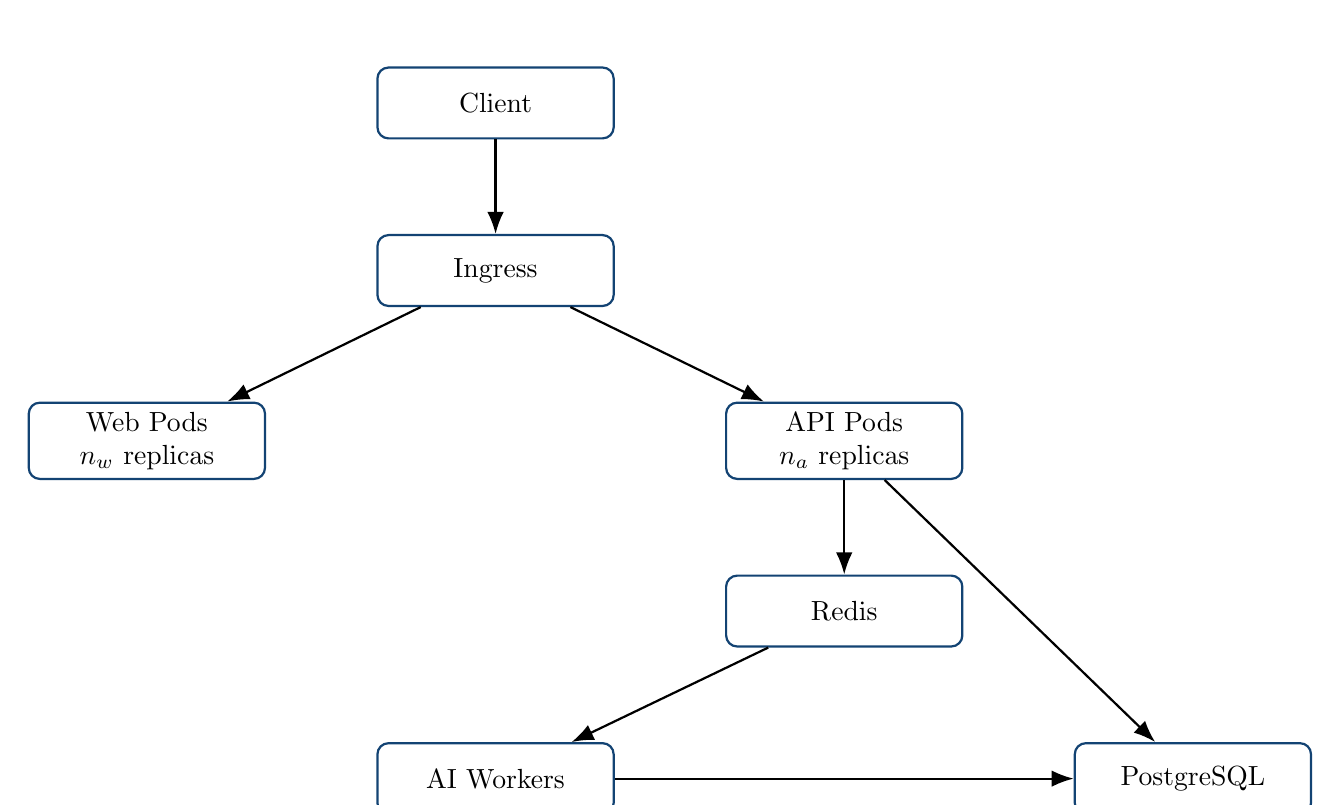
\begin{tikzpicture}[
    node distance=1.2cm and 1.4cm,
    box/.style={
        rectangle,
        rounded corners,
        draw=ADGBlue,
        thick,
        minimum width=3cm,
        minimum height=0.9cm,
        align=center
    },
    arrow/.style={-{Latex[length=2.8mm]}, thick}
]

\node[box] (internet) {Client};
\node[box, below=of internet] (ingress) {Ingress};
\node[box, below left=of ingress] (web) {Web Pods\\$n_w$ replicas};
\node[box, below right=of ingress] (api) {API Pods\\$n_a$ replicas};

\node[box, below=of api] (redis) {Redis};
\node[box, below left=of redis] (worker) {AI Workers};
\node[box, below right=of redis] (db) {PostgreSQL};

\draw[arrow] (internet) -- (ingress);
\draw[arrow] (ingress) -- (web);
\draw[arrow] (ingress) -- (api);
\draw[arrow] (api) -- (redis);
\draw[arrow] (api) -- (db);
\draw[arrow] (redis) -- (worker);
\draw[arrow] (worker) -- (db);

\end{tikzpicture}

\caption{Illustrative Kubernetes deployment.}
\end{figure}

% ============================================================
\section{Horizontal Scaling}
% ============================================================

For \(n\) API replicas with individual effective capacities \(C_i\):

\[
C_{ideal}
=
\sum_{i=1}^{n}C_i.
\]

Actual capacity satisfies approximately:

\[
C_{actual}
\leq
\sum_{i=1}^{n}C_i
\]

because of shared bottlenecks including:

\begin{itemize}
    \item PostgreSQL;
    \item Redis;
    \item network bandwidth;
    \item connection pools;
    \item storage;
    \item AI inference capacity.
\end{itemize}

Therefore the system does not assume perfect linear scaling.

% ============================================================
\section{Horizontal Pod Autoscaling}
% ============================================================

Suppose:

\[
U_c
\]

is current average CPU utilisation and

\[
U_t
\]

is target utilisation.

A simplified desired replica estimate is:

\[
N_{desired}
=
\left\lceil
N_{current}
\frac{U_c}{U_t}
\right\rceil.
\]

For example:

\[
N_{current}=3,
\quad
U_c=80\%,
\quad
U_t=60\%.
\]

Then:

\[
N_{desired}
=
\left\lceil
3
\frac{0.80}{0.60}
\right\rceil
=
\lceil4\rceil
=
4.
\]

% ============================================================
\section{Failure Behaviour}
% ============================================================

\subsection{Redis Failure}

If Redis becomes unavailable:

\begin{itemize}
    \item authoritative dispute records remain in PostgreSQL;
    \item non-essential caching may degrade;
    \item AI/background jobs may pause;
    \item rate-limiting behaviour must fail according to explicit policy.
\end{itemize}

\subsection{Ollama Failure}

If Ollama becomes unavailable:

\[
CoreDisputeWorkflow = Available.
\]

AI functionality shall degrade gracefully.

\subsection{Worker Failure}

A worker crash must not corrupt dispute state.

Jobs shall be retried only where operations are safe and idempotent.

% ============================================================
\section{Testing Strategy}
% ============================================================

Testing shall include:

\begin{enumerate}
    \item unit tests;
    \item integration tests;
    \item API tests;
    \item database tests;
    \item frontend component tests;
    \item end-to-end tests;
    \item authorisation tests;
    \item concurrency tests;
    \item AI schema validation tests.
\end{enumerate}

% ============================================================
\section{Critical Test Cases}
% ============================================================

The test suite shall verify at minimum:

\begin{itemize}
    \item a customer can view their own transactions;
    \item a customer cannot view another customer's transaction;
    \item a customer can dispute an eligible transaction;
    \item duplicate active disputes are rejected;
    \item invalid state transitions are rejected;
    \item analyst-only endpoints reject customers;
    \item idempotent retries do not create duplicate disputes;
    \item concurrent dispute creation preserves uniqueness;
    \item AI failure does not break core dispute functionality;
    \item malformed AI output is rejected;
    \item unauthorised agent tools cannot execute.
\end{itemize}

% ============================================================
\section{Concurrency Test}
% ============================================================

Suppose \(m\) requests simultaneously attempt to dispute transaction
\(t\).

Let:

\[
D_t
=
\{
d\in\mathcal{D}:d.transaction=t
\land
d.status\in S_A
\}.
\]

After all requests complete, the invariant must remain:

\[
|D_t|\leq1.
\]

This shall be verified through an automated concurrency test.

% ============================================================
\section{Property-Based Testing}
% ============================================================

The state machine is suitable for property-based testing.

For every generated state/event pair:

\[
(s,e),
\]

the implementation should satisfy:

\[
Implementation(s,e)
=
T(s,e).
\]

Furthermore, no generated sequence of valid application operations
should violate:

\[
ActiveDisputes(transaction)\leq1.
\]

% ============================================================
\section{Performance Testing}
% ============================================================

Benchmark scenarios should include:

\begin{itemize}
    \item transaction list retrieval;
    \item transaction detail retrieval;
    \item dispute creation;
    \item dispute timeline retrieval;
    \item analyst queue retrieval.
\end{itemize}

Results shall report:

\[
Throughput,
\quad
P_{50},
\quad
P_{95},
\quad
P_{99},
\quad
ErrorRate.
\]

Any benchmark claims shall include:

\begin{itemize}
    \item hardware;
    \item dataset size;
    \item concurrent users;
    \item test duration;
    \item software configuration.
\end{itemize}

% ============================================================
\section{CI/CD}
% ============================================================

The repository should contain automated CI steps for:

\begin{enumerate}
    \item Rust formatting;
    \item Rust linting;
    \item Rust tests;
    \item frontend linting;
    \item frontend tests;
    \item production frontend build;
    \item Docker image build;
    \item optional vulnerability scanning.
\end{enumerate}

A failing test shall prevent successful CI completion.

% ============================================================
\section{Configuration and Secrets}
% ============================================================

Secrets shall never be committed to Git.

The repository may provide:

\begin{lstlisting}
.env.example
\end{lstlisting}

containing placeholder configuration.

Sensitive values include:

\begin{itemize}
    \item database credentials;
    \item signing keys;
    \item API secrets;
    \item object storage credentials.
\end{itemize}

Kubernetes manifests shall reference secrets rather than embedding
production values.

% ============================================================
\section{Example Customer Journey}
% ============================================================

Consider a customer with transaction:

\[
x = R8750.00.
\]

Suppose their historical mean is:

\[
\bar{x}=R643.00
\]

with standard deviation:

\[
s=R920.00.
\]

Then:

\[
z
=
\frac{8750-643}{920}.
\]

First calculate:

\[
8750-643=8107.
\]

Therefore:

\[
z
=
\frac{8107}{920}.
\]

Hence:

\[
z
\approx8.81.
\]

Thus:

\[
|z|\approx8.81>3.
\]

The system may therefore display:

\begin{quote}
Transaction amount is highly unusual relative to the customer's
historical transaction amounts.
\end{quote}

This does not establish fraud.

The customer then submits a dispute.

The backend verifies:

\[
Owner(customer,transaction)=true.
\]

It verifies:

\[
ActiveDisputes(transaction)=0.
\]

It then atomically creates:

\[
Dispute
+
DisputeEvent
+
AuditEvent.
\]

The customer receives a reference such as:

\begin{center}
\texttt{DSP-2026-000184}
\end{center}

% ============================================================
\section{Example AI Investigation}
% ============================================================

After dispute creation, an asynchronous job may start.

Iteration \(0\):

\[
A_0=(C_0,\emptyset,B_0).
\]

The agent requests transaction information:

\[
\tau_0=get\_transaction.
\]

The result is added:

\[
O_1=O_0\cup\{transaction\}.
\]

The agent requests deterministic risk signals:

\[
\tau_1=get\_risk\_signals.
\]

Then:

\[
O_2
=
O_1
\cup
\{
amount,
velocity,
geographic,
history
\}.
\]

If enough information exists:

\[
Complete(A_2)=true.
\]

The model produces a structured summary.

No dispute decision is automatically performed.

% ============================================================
\section{Example Analyst Interface}
% ============================================================

The analyst may see:

\begin{lstlisting}
CASE: DSP-2026-000184

Transaction
-----------
Merchant:       Example Electronics
Amount:         R8,750.00
Date:           30 October 2026

Risk Signals
------------
Amount anomaly:       HIGH
Velocity anomaly:     LOW
Geographic anomaly:   MODERATE
Historical anomaly:   HIGH

AI Assistance
-------------
Suggested category:
CARD_NOT_PRESENT / UNRECOGNISED

Recommendation:
MANUAL REVIEW

Case Status
-----------
UNDER_REVIEW
\end{lstlisting}

The analyst, not the AI system, performs the authorised workflow action.

% ============================================================
\section{Dispute Timeline}
% ============================================================

A typical timeline may be:

\begin{lstlisting}
30 Oct 2026 14:32
* Dispute submitted

30 Oct 2026 14:32
* Dispute acknowledged

31 Oct 2026 09:14
* Review started

31 Oct 2026 09:17
* Evidence requested

01 Nov 2026 10:02
* Evidence received

01 Nov 2026 13:20
* Investigation started

02 Nov 2026 11:10
* Analyst decision recorded
\end{lstlisting}

Each timeline entry is derived from persisted dispute events rather than
invented client-side state.

% ============================================================
\section{Production Engineering Principles}
% ============================================================

The implementation shall follow these principles:

\begin{enumerate}
    \item PostgreSQL is authoritative.
    \item Redis is disposable.
    \item AI is optional.
    \item AI does not determine financial outcomes.
    \item Every protected resource is authorised server-side.
    \item Critical invariants are enforced at multiple layers.
    \item Monetary arithmetic is exact.
    \item Retries are expected.
    \item Concurrent requests are expected.
    \item Every important state transition is auditable.
    \item Services expose health and readiness.
    \item Failure of optional components must degrade gracefully.
    \item Local execution must remain simple.
\end{enumerate}

% ============================================================
\section{Engineering Trade-Offs}
% ============================================================

\subsection{Why Rust?}

Rust is not selected solely because of raw benchmark performance.

The design benefits include:

\begin{itemize}
    \item memory safety;
    \item strong compile-time guarantees;
    \item explicit error handling;
    \item predictable resource usage;
    \item high-performance asynchronous execution;
    \item strong type modelling for domain states.
\end{itemize}

\subsection{Why PostgreSQL?}

The dispute workflow requires strong transactional semantics and
relational integrity.

PostgreSQL provides:

\begin{itemize}
    \item ACID transactions;
    \item constraints;
    \item indexes;
    \item row locking;
    \item mature relational querying.
\end{itemize}

\subsection{Why Redis?}

Redis supports ephemeral performance and coordination workloads without
replacing PostgreSQL as the authoritative database.

\subsection{Why Ollama?}

Ollama enables local model execution and allows AI functionality to be
demonstrated without coupling core dispute processing to a remote LLM
provider.

\subsection{Why Kubernetes?}

Kubernetes is included to demonstrate a possible scalable deployment
model.

It is deliberately not required for local evaluation.

Docker Compose remains the simplest supported execution path.

% ============================================================
\section{Definition of Done}
% ============================================================

The project is complete when:

\begin{enumerate}
    \item a fresh clone can be started according to the README;
    \item Docker builds successfully;
    \item seeded users can authenticate;
    \item customers can view mock transactions;
    \item customers can submit disputes;
    \item duplicate disputes are prevented;
    \item customers can view dispute timelines;
    \item analysts can review disputes;
    \item authorised state transitions work;
    \item unauthorised transitions fail;
    \item audit events are persisted;
    \item deterministic risk indicators are visible;
    \item optional AI analysis works when Ollama is available;
    \item the system remains usable when AI is unavailable;
    \item automated tests pass;
    \item Kubernetes manifests are documented if included.
\end{enumerate}

% ============================================================
\section{Presentation Strategy}
% ============================================================

The demonstration should proceed in the following order:

\begin{enumerate}
    \item Present the business problem.
    \item Present the architecture.
    \item Login as a customer.
    \item View transactions.
    \item Open an unusual transaction.
    \item Explain mathematical risk indicators.
    \item Submit a dispute.
    \item Demonstrate duplicate prevention.
    \item Display the dispute timeline.
    \item Login as an analyst.
    \item Review the case.
    \item Demonstrate AI-assisted analysis.
    \item Demonstrate the bounded agent execution events.
    \item Perform an authorised state transition.
    \item Display the audit trail.
    \item Explain PostgreSQL consistency.
    \item Explain Redis responsibilities.
    \item Demonstrate tests.
    \item Demonstrate Docker.
    \item Present the optional Kubernetes deployment.
\end{enumerate}

% ============================================================
\section{Final Architecture Principle}
% ============================================================

The overall system can be summarised as:

\[
\boxed{
\begin{array}{c}
\text{Customer / Analyst} \\[3pt]
\downarrow \\[3pt]
\text{Next.js} \\[3pt]
\downarrow \\[3pt]
\text{Rust / Axum} \\[3pt]
\downarrow \\[3pt]
\text{Domain Rules + Mathematical Risk Engine} \\[3pt]
\downarrow \\[3pt]
\text{PostgreSQL + Redis} \\[3pt]
\downarrow \\[3pt]
\text{Ollama + Bounded AI Agent} \\[3pt]
\downarrow \\[3pt]
\text{Human Decision}
\end{array}
}
\]

with deployment provided through:

\[
\boxed{
Docker
\rightarrow
Docker\ Compose
\rightarrow
Optional\ Kubernetes
}
\]

The central design philosophy remains:

\[
\boxed{
Correctness
>
Complexity
}
\]

\[
\boxed{
Security
>
Convenience
}
\]

and

\[
\boxed{
AI\ Assists
\quad
Human\ Decides.
}
\]

% ============================================================
\section{Conclusion}
% ============================================================

ADGSTUDIOS DisputeGuard demonstrates how a relatively small card
dispute brief can be engineered as a realistic financial-services
software system.

The architecture deliberately separates deterministic domain rules,
mathematical risk analysis, transactional persistence, ephemeral
coordination and generative AI.

The result is intended to demonstrate not merely the ability to build
a full-stack interface, but the ability to reason about:

\begin{itemize}
    \item correctness;
    \item security;
    \item mathematics;
    \item concurrency;
    \item distributed systems;
    \item artificial intelligence;
    \item observability;
    \item scalability;
    \item testing;
    \item production deployment.
\end{itemize}

\begin{center}
\vspace{1cm}
\textbf{\Large ADGSTUDIOS DisputeGuard}

\vspace{0.3cm}

\textit{Secure. Explainable. Auditable. Scalable.}
\end{center}

\end{document}